\documentclass{examen}

\begin{document}
\modulo{Lenguajes de marcas. Recuperaci�n primera evaluaci�n}

\pregunta{Crear en HTML un formulario como el mostrado en la figura}{5}
\begin{figure}[h]
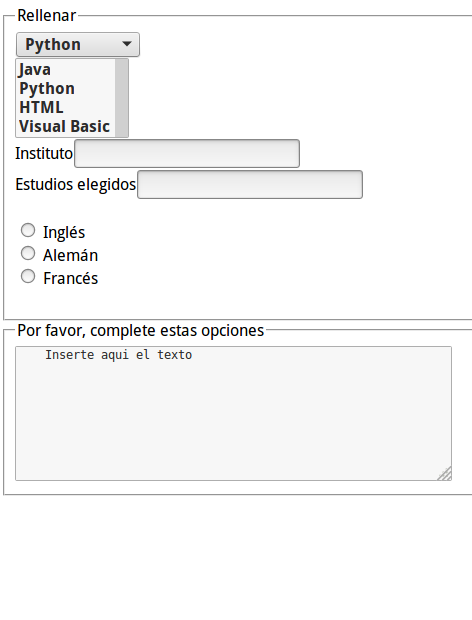
\includegraphics[scale=0.5]{examen-img/foto_formulario_11.png}
\end{figure}
\break

\pregunta{Crea una p�gina HTML que se modifique con CSS y que contenga los siguientes
elementos
\begin{itemize}
\item{Dos encabezamientos h1 y dos encabezamientos h2. Modifica con CSS y el atributo
{\tt class} su aspecto para que aparezcan escritos con un color distinto.}
\item{Crea una lista numerada con 3 elementos. Modifica el tipo de letra del primero y el tercero usando {\tt id}}
\item{Crea una tabla de 3 filas y 4 columnas. Dentro de cada celda puedes escribir cualquier cosa. Usando CSS y la t�cnica que prefieras modifica el fondo de las celdas de la columna que quieras}
\end{itemize}
}{5	}

\end{document}
